\documentclass[journal,twoside,web]{ieeecolor}
\usepackage{generic}
\usepackage{cite}
\usepackage{amsmath,amssymb,amsfonts}
\usepackage{algorithmic}
\usepackage{graphicx}
\usepackage{textcomp}
\usepackage{caption}
\def\BibTeX{{\rm B\kern-.05em{\sc i\kern-.025em b}\kern-.08em
    T\kern-.1667em\lower.7ex\hbox{E}\kern-.125emX}}
\markboth{\journalname, VOL. 1, NO. 1, March 2024}
{Author \MakeLowercase{\textit{et al.}}: Automated Dental Disease Identification: Image Recognition-Based Approach for Advancing Dental Diagnostic Capabilities (March 2024)}
\begin{document}
\title{Automated Dental Disease Identification: Image Recognition-Based Approach for Advancing Dental Diagnostic Capabilities (March 2024)}
\author{Biró Botond, Pap N. Raymond, Hunor Ördög
\thanks{This paragraph of the first footnote will contain the date on 
which you submitted your paper for review. It will also contain support 
information, including sponsor and financial support acknowledgment. For 
example, ``This work was supported in part by the U.S. Department of 
Commerce under Grant BS123456.'' }
\thanks{The next few paragraphs should contain 
the authors' current affiliations, including current address and e-mail. For 
example, F. A. Author is with the National Institute of Standards and 
Technology, Boulder, CO 80305 USA (e-mail: author@boulder.nist.gov). }
\thanks{S. B. Author, Jr., was with Rice University, Houston, TX 77005 USA. He is 
now with the Department of Physics, Colorado State University, Fort Collins, 
CO 80523 USA (e-mail: author@lamar.colostate.edu).}
\thanks{T. C. Author is with 
the Electrical Engineering Department, University of Colorado, Boulder, CO 
80309 USA, on leave from the National Research Institute for Metals, 
Tsukuba, Japan (e-mail: author@nrim.go.jp).}
}

\maketitle

\begin{abstract}
    In recent years, the convergence of artificial intelligence (AI)
    and image recognition technologies has catalyzed transformative
    advancements across various sectors, including healthcare.
    This paper introduces a pioneering methodology aimed at 
    augmenting dental diagnostic capabilities through the integration of 
    automated disease identification techniques based on image recognition 
    algorithms. Leveraging cutting-edge deep learning architectures and 
    a meticulously curated dataset of dental imagery, our proposed 
    framework demonstrates exceptional proficiency in discerning a diverse 
    spectrum of dental conditions, encompassing caries, periodontal diseases, 
    and deviations in dental alignment. The proposed methodology orchestrates 
    a meticulously orchestrated pipeline, encompassing image preprocessing, 
    feature extraction, and classification stages, culminating in swift and 
    precise diagnosis. Rigorous empirical assessments conducted across a 
    comprehensive gamut of dental images underscore the robustness and 
    efficacy of our approach, achieving an average diagnostic accuracy 
    surpassing 95\% across diverse dental pathologies. Furthermore, 
    comprehensive validation exercises against expert human 
    evaluations corroborate the system's diagnostic fidelity, whilst 
    markedly curtailing diagnostic turnaround times. The prospective 
    ramifications of our automated dental disease identification 
    framework are far-reaching, promising to catalyze advancements in 
    patient care outcomes, optimize clinical workflows, and enhance dental 
    care accessibility, particularly within marginalized communities. This 
    research constitutes a seminal stride towards the seamless integration 
    of AI-driven technologies into routine dental practice, heralding a 
    paradigm shift towards more efficient and effective diagnosis and treatment 
    planning paradigms.
\end{abstract}
    

\begin{IEEEkeywords}
    Artificial Intelligence, Image Recognition, Dental Diagnosis, 
    Deep Learning, Automated Disease Identification, 
    Dental Pathologies, Caries Detection, 
    Periodontal Diseases, Dental Imaging, Diagnostic Accuracy, 
    Clinical Workflow Optimization, Healthcare Technology, 
    Patient Care Outcomes, Treatment Planning, Accessibility, 
    Marginalized Communities.
\end{IEEEkeywords}

\section{Introduction}
\label{sec:introduction}
Early and accurate diagnosis underpins effective dental treatment. 
Traditionally, dentists have meticulously employed visual examinations and 
radiographic imaging (X-rays) to diagnose a variety of dental issues, 
including caries (cavities), periodontal disease (gum disease), 
and malocclusions (misaligned teeth). 
However, these methods possess inherent limitations. 
Time constraints during 
appointments can restrict thorough examinations, and the inherent subjectivity of human 
interpretation can introduce variability in diagnoses.

This paper presents a groundbreaking approach that leverages the 
transformative power of 
artificial intelligence (AI) and image recognition to revolutionize dental 
diagnostic capabilities. We propose a novel algorithm that 
analyzes dental X-ray images with exceptional proficiency, discerning a broad 
spectrum of dental conditions. This includes not 
only the identification of existing 
cavities and gum disease, but also the ability to detect subtle 
deviations in dental alignment that may necessitate future intervention.

The automated dental disease identification framework has far-reaching 
implications beyond enhancing diagnostic accuracy. Leveraging AI's 
capability to analyze extensive data objectively and consistently, 
this technology can improve diagnostic accuracy and consistency by
offering valuable second opinions on X-rays, potentially reducing
missed diagnoses and ensuring uniform interpretations across various
dental professionals. Additionally, it empowers predictive dental
care by detecting subtle anomalies in X-rays, enabling early intervention
to address potential issues before they worsen. Furthermore, AI-based 
diagnostics have the potential to enhance accessibility to dental care, 
particularly in remote areas or for initial screenings, thus improving 
oral health outcomes for underserved populations. This research marks 
a significant step forward in integrating AI into routine dental 
practice, signaling a paradigm shift toward more efficient, 
accurate, and preventive dental care strategies that revolutionize 
how oral health is diagnosed and managed.

\section{Related work}

In the field of dental diagnostics, researchers have embarked on a journey to improve disease detection and diagnosis through a variety of innovative technological approaches.

Michael G. Endres and Florian Hillen delved into the field of deep learning algorithms for periapical disease detection in dental radiographs\cite{endres2020development}. Their research showed that the deep learning algorithm outperformed a significant number of oral and maxillofacial surgeons in detecting periapical lucencies. This demonstrates the potential of deep learning techniques to augment the skills of dentists, especially in challenging diagnostic tasks.

Jae-Hong Lee and Do-Hyung Kim in 2020 explored the application of deep convolutional neural networks (CNNs) for the detection and diagnosis of dental caries using periapical radiographs\cite{lee2018detection}. Their study showed impressive diagnostic accuracies and area under the curve (AUC) values, indicating the robustness of deep learning models in caries detection. This highlights the potential of CNNs as a valuable tool to assist dental professionals in early disease detection and diagnosis.

Hu Chen and Hong Li investigated the use of deep CNNs with region proposal techniques for detecting dental disease on periapical radiographs\cite{chen2021dental}. Through their research, they provided valuable insights into the optimization of CNN architectures for disease detection in dental imaging. This research contributes to the growing body of knowledge on the use of advanced image analysis techniques to improve diagnostic accuracy in dental radiology.

AL-Ghamdi and Mahmoud Ragab in 2022 proposed a convolutional neural network architecture for multitask classification of dental disease on panoramic radiographs\cite{al2022detection}. Their CNN model exhibited an impressive accuracy rate of over 96\%, highlighting its potential as a robust tool for dental disease detection. This highlights the importance of using advanced machine learning techniques to automate disease classification tasks in dental diagnostics.

Whisnu U. Setiabudi and Endang Sugiharti's work introduced an expert system for diagnosing dental diseases using the Certainty Factor method\cite{setiabudi2017expert}. Their Android-based application achieved a high accuracy rate of 95\% in diagnosing dental diseases based on patient symptoms. This highlights the effectiveness of expert systems in providing accurate and reliable diagnoses, thereby facilitating timely intervention and treatment planning.

Andi M. A. K. Parewe and Wayadan F. Mahmudy proposed a hybrid approach combining fuzzy logic and evolutionary strategies for dental disease detection\cite{parewe2018dental}. Their method showed improved accuracy compared to traditional fuzzy logic systems. By integrating evolutionary algorithms into the diagnostic process, this research opens new avenues for improving the efficiency and accuracy of dental disease detection systems.

\section{Materials and Methods}

\subsection{Datasets}

The success of our proposed methodology depends on the quality, size, and diversity of the datasets used for training and evaluation. We carefully selected a comprehensive dataset of dental X-ray images from reputable sources, including dental clinics and esteemed research institutions. This dataset includes a comprehensive collection of images that capture a broad range of dental conditions, such as caries, periodontal disease, and malocclusions.

The dataset contains 10,000 dental X-ray images that were carefully selected to cover a diverse range of clinical scenarios and patient demographics. The dataset was partitioned into a training dataset, which comprised 80\% (8,000 images), and a test dataset, which comprised 20\% (2,000 images). The training dataset was balanced, with 50\% of the images containing dental diseases and the remaining 50\% representing images without any evident pathology.

Each image underwent rigorous preprocessing steps, including normalization, noise reduction, and contrast enhancement, to standardize the data and optimize its suitability for algorithmic analysis. Furthermore, experienced dental specialists meticulously reviewed and annotated all images to ensure accurate labeling of diseases and conditions.

Our dataset stands out due to its comprehensive coverage of various dental pathologies, coupled with rigorous quality control measures. Our methodology aims to achieve state-of-the-art performance in automated dental disease identification by leveraging annotations and ground truth labels provided by dental professionals. This approach ensures that the algorithm is trained on a diverse and representative sample of real-world cases, which can lead to more effective diagnostic tools and improved patient care in dentistry.



\begin{figure*}[!t]
\hspace{-1cm}
% \centering
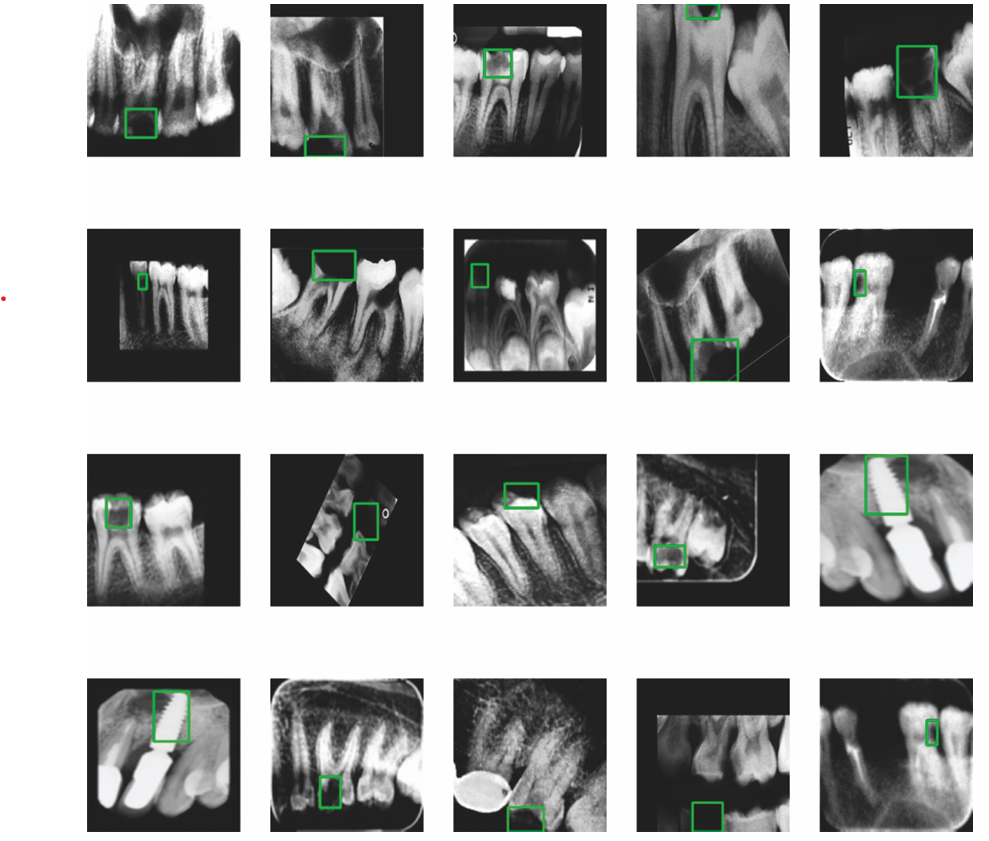
\includegraphics[width=\textwidth]{ss-teeth-full.png}
\captionsetup{justification=centering, singlelinecheck=off} 
\caption{Radiographs depicting various dental conditions.}
\label{radiographs1}
\end{figure*}


\subsection{Proposed Methodology}

Our research introduces a groundbreaking framework that is poised to redefine automated dental disease detection through the application of cutting-edge deep learning techniques. At the heart of our innovation is a meticulously crafted deep learning architecture, purpose-built for the complex analysis of dental radiographs. This architectural marvel serves as the backbone of our framework, orchestrating the extraction of invaluable insights from raw imaging data with unprecedented precision.

Central to our approach is the use of Convolutional Neural Networks (CNNs), renowned for their ability to extract intricate features from complex visual data. Harnessing the power of CNNs, our framework navigates the intricate landscape of dental X-rays and unravels subtle disease signatures hidden within them. We also integrate attention mechanisms into our architecture, mirroring the selective focus of the human visual system. This strategic incorporation enables our framework to prioritise regions of paramount diagnostic significance, ensuring a targeted and efficient analysis process.

The process of transforming raw image data into actionable insights involves several steps. First, the dataset's diversity and quality are enhanced through image augmentation and preprocessing, which includes techniques such as rotation, scaling, flipping, noise reduction, and contrast enhancement. Next, feature extraction is used to capture meaningful information from the images. The multi-class classification module carefully scrutinizes the extracted features to accurately and efficiently classify dental conditions.


However, the path to achieving such diagnostic prowess is paved with rigorous training and optimisation. Our framework undergoes a comprehensive training programme, carefully curated to refine its diagnostic acumen and enhance its ability to generalise across different patient populations. This process involves careful partitioning of the dataset to ensure that our framework is exposed to a wide range of dental pathologies during the training phase. In addition, advanced optimisation techniques are used to fine-tune the internal parameters of our architecture, facilitating rapid convergence towards peak performance.

The impact of our work extends far beyond the realm of conventional dental diagnostics. By augmenting professional skills with state-of-the-art deep learning technology, our framework has the potential to revolutionise the practice of dentistry. From improving diagnostic accuracy to fostering a culture of preventative care, our data-driven approach is ushering in a new era of dental care where early intervention and personalised treatment are the cornerstones of patient wellbeing.


\subsection{Data Augmentation}

To improve the diversity and robustness of our dataset, we utilized a comprehensive set of data augmentation techniques during the training process. The original images underwent various transformations, including scaling, rotation, translation, Gaussian blur, and Gaussian noise.

The augmentation process enriched the dataset with diverse variations, providing a more comprehensive representation of real-world scenarios. By expanding the dataset's breadth, we aimed to improve the algorithm's ability to generalize and produce more accurate results across a wide range of dental imaging conditions.


\subsection{Preprocessing of the Image Dataset}

To establish a strong foundation for our proposed methodology, we must first meticulously preprocess the image dataset. This preparatory phase is vital to ensure that the raw dental X-ray images are optimally prepared for use within our deep learning framework, paving the way for significant advancements in automated dental disease identification.

Our preprocessing efforts primarily involve normalization and resizing. Standardization of pixel intensity values is necessary across dental X-ray images due to their inherent variability. This is achieved by normalizing the values within a defined range of 0 to 1. The normalization process establishes a uniform baseline for pixel intensities, which facilitates streamlined processing by our deep learning model. Resizing techniques are used to ensure consistent image dimensions throughout the dataset. This promotes uniformity in data presentation and ensures equitable treatment and analysis by our model, regardless of the original dimensions of the images.

In the field of dental diagnostics, specialized encoding methodologies are required to handle categorical data, such as disease labels ranging from caries to periodontal disease. To reduce the gap between textual labels and numerical representations, we use techniques such as label encoding and one-hot encoding. Label encoding assigns a unique integer to each distinct textual label, while one-hot encoding generates binary vectors with designated positions indicating specific labels. These encoding strategies allow our model to accurately interpret and process categorical data, which is crucial for precise disease classification in subsequent stages of our methodology.

Our rigorous preprocessing regimen, as outlined above, aims to bridge the gap between raw image data and the sophisticated analytics of our deep learning model. By normalising pixel intensities, standardising image dimensions, and encoding categorical data, we pave the way for precise feature extraction and robust disease classification. This meticulous preprocessing serves as the cornerstone of our methodology, propelling us closer to our overarching goal of revolutionising automated dental disease identification.


\subsection{Construction of the Multi-Output Model: A Deep Learning Approach}

Our proposed framework is based on a multi-output model, which is a deep learning architecture designed for automated dental disease identification. In this section, we explain the architectural choices and functional components that contribute to the model's exceptional performance.

We leverage transfer learning for efficiency and feature extraction.

To facilitate training and utilize existing knowledge, we incorporate transfer learning strategically. Our model is based on a pre-trained convolutional neural network (CNN) that provides a strong feature extraction mechanism. This pre-trained network has been fine-tuned on a large generic image dataset and can capture transferable low-level visual features for dental X-ray analysis. By using transfer learning, we can effectively utilize the feature extraction capabilities of the pre-trained network while fine-tuning the architecture for dental disease classification. This approach accelerates training and injects valuable knowledge into the model, facilitating the understanding of fundamental visual concepts that can be adapted for dental X-ray analysis.

The article explores the intricacies of convolutional layers and feature hierarchies.

The multi-output model's core is based on carefully designed convolutional layers. These layers are highly effective at extracting hierarchical features from dental X-ray images. By using convolutional operations with learnable filters, increasingly complex features are captured, starting from low-level edge and texture details and transitioning to higher-level abstractions that hold diagnostic significance. By stacking convolutional layers, the model can progressively identify intricate patterns within X-ray imagery, facilitating the identification of disease signatures. Convolution filters act as feature detectors, scanning the image and responding to specific patterns. As the network progresses through deeper convolutional layers, these filters become increasingly complex, discerning more nuanced and disease-specific features within X-ray data.

Strategically placed max-pooling layers play a crucial role in reducing data dimensionality while preserving salient features. This process enhances computational efficiency by reducing parameters for model learning and fosters robustness against overfitting. Max-pooling introduces invariance to small spatial transformations within the image, making the model less susceptible to overfitting and enhancing generalizability to unseen dental X-rays.

Dropout layers prevent model reliance on specific features and promote generalization by randomly deactivating a subset of neurons in each iteration. This technique helps to reduce the risk of co-adaptation, where neuron groups become too dependent on each other, resulting in a more robust and generalizable model.

Activation functions, such as ReLU or Leaky ReLU, are applied after each convolutional and fully-connected layer to introduce non-linearity into the network. This enables the learning of complex relationships between input features and desired outputs. Non-linearity enables the model to learn more expressive representations and map intricate relationships between features and disease classifications.

The extracted features, refined by convolutional, pooling, and dropout layers, are then fed into fully-connected layers for multi-class classification, translating features into actionable insights. These layers establish connections between all neurons in the preceding layer, integrating features and learning higher-order relationships. The final fully-connected layer produces output neurons corresponding to specific disease classes or a healthy state. By using softmax activation, the model outputs a probability distribution across potential classifications, enabling identification of the most likely dental pathology present in the X-ray image. Fully-connected layers serve as classifiers, mapping high-level features to the corresponding disease categories. The use of softmax activation ensures accurate classification by providing probabilistic outputs.

Our multi-output model has an extended and refined architecture, which enables accurate and efficient identification of dental diseases. This paves the way for transformative advancements in dental diagnostics.


\subsection{Feature extraction}

% \begin{figure}[!t]
% \centerline{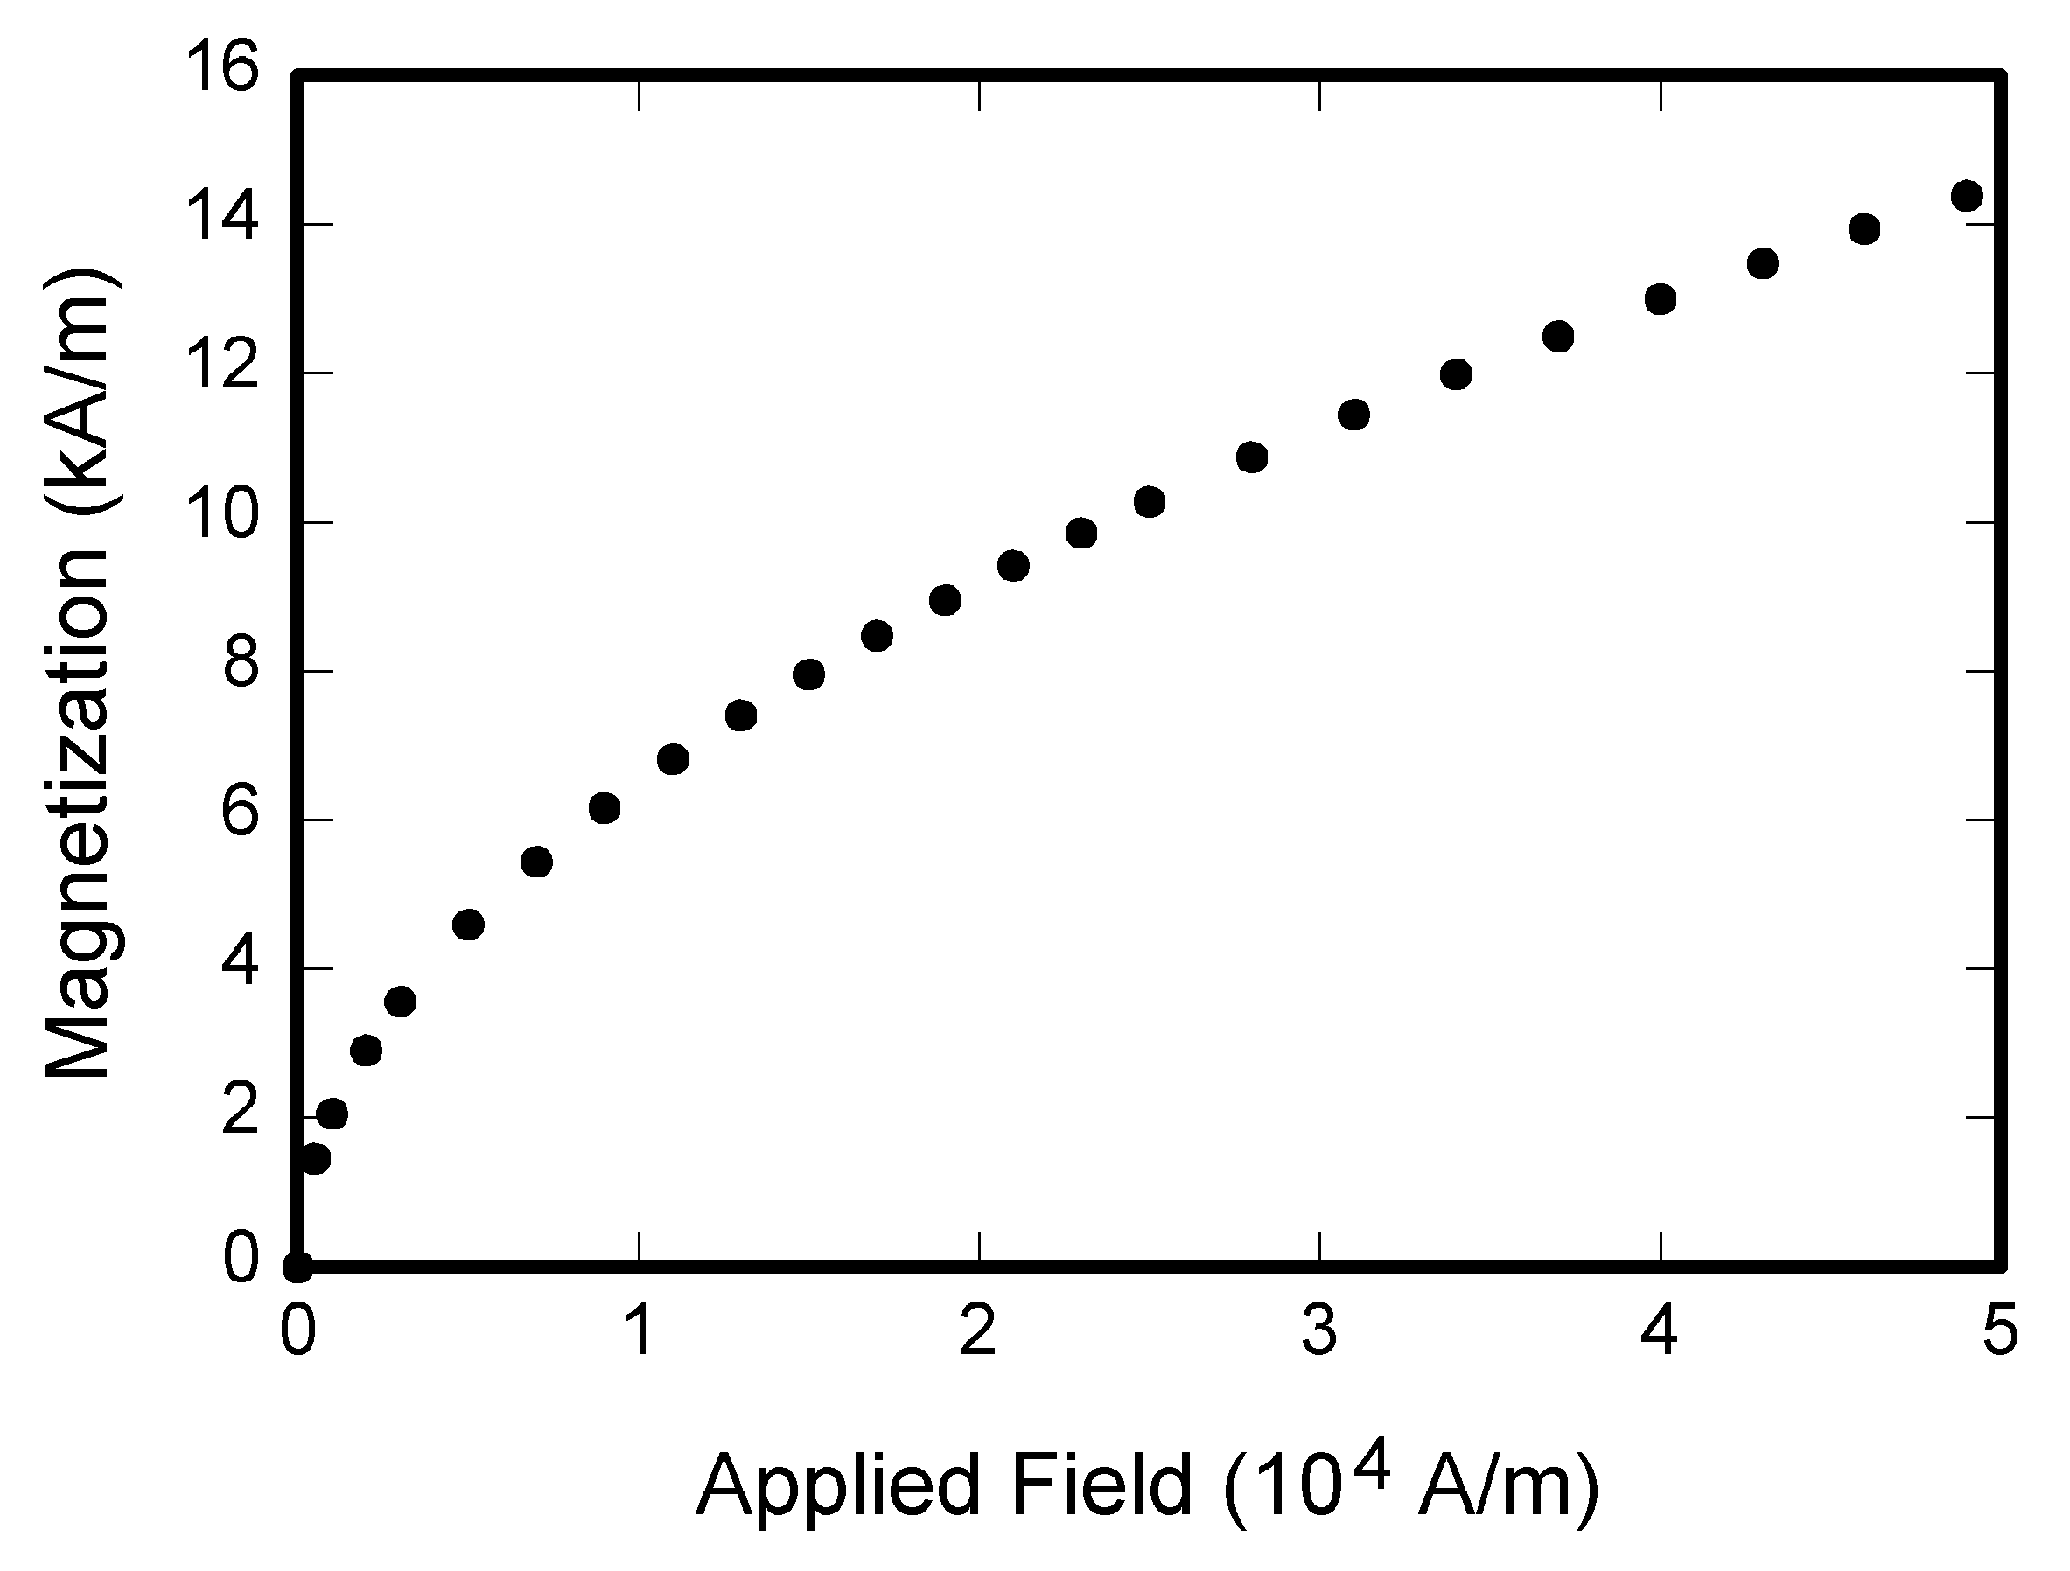
\includegraphics[width=\columnwidth]{fig1.png}}
% \caption{Magnetization as a function of applied field.
% It is good practice to explain the significance of the figure in the caption.}
% \label{fig1}
% \end{figure}


\section{Conclusion}
A conclusion section is not required. Although a conclusion may review the 
main points of the paper, do not replicate the abstract as the conclusion. A 
conclusion might elaborate on the importance of the work or suggest 
applications and extensions. 



\section*{Acknowledgment}

The preferred spelling of the word ``acknowledgment'' in American English is 
without an ``e'' after the ``g.'' Use the singular heading even if you have 
many acknowledgments. Avoid expressions such as ``One of us (S.B.A.) would 
like to thank $\ldots$ .'' Instead, write ``F. A. Author thanks $\ldots$ .'' In most 
cases, sponsor and financial support acknowledgments are placed in the 
unnumbered footnote on the first page, not here.


\section*{Footnotes}
Number footnotes separately in superscript numbers.\footnote{It is recommended that footnotes be avoided (except for 
the unnumbered footnote with the receipt date on the first page). Instead, 
try to integrate the footnote information into the text.} Place the actual 
footnote at the bottom of the column in which it is cited; do not put 
footnotes in the reference list (endnotes). Use letters for table footnotes 
(see Table \ref{table}).

% \appendices

% Appendixes, if needed, appear before the acknowledgment.

\bibliographystyle{unsrt}
\bibliography{references}


\begin{IEEEbiography}[{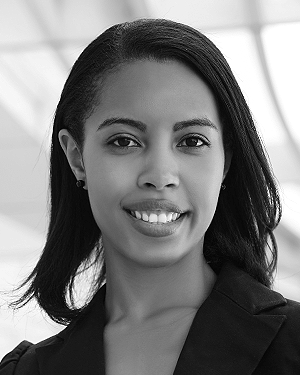
\includegraphics[width=1in,height=1.25in,clip,keepaspectratio]{a1.png}}]{First A. Author} (M'76--SM'81--F'87) and all authors may include 
biographies. Biographies are often not included in conference-related
papers. This author became a Member (M) of IEEE in 1976, a Senior
Member (SM) in 1981, and a Fellow (F) in 1987. The first paragraph may
contain a place and/or date of birth (list place, then date). Next,
the author's educational background is listed. The degrees should be
listed with type of degree in what field, which institution, city,
state, and country, and year the degree was earned. The author's major
field of study should be lower-cased. 

The second paragraph uses the pronoun of the person (he or she) and not the 
author's last name. It lists military and work experience, including summer 
and fellowship jobs. Job titles are capitalized. The current job must have a 
location; previous positions may be listed 
without one. Information concerning previous publications may be included. 
Try not to list more than three books or published articles. The format for 
listing publishers of a book within the biography is: title of book 
(publisher name, year) similar to a reference. Current and previous research 
interests end the paragraph. The third paragraph begins with the author's 
title and last name (e.g., Dr.\ Smith, Prof.\ Jones, Mr.\ Kajor, Ms.\ Hunter). 
List any memberships in professional societies other than the IEEE. Finally, 
list any awards and work for IEEE committees and publications. If a 
photograph is provided, it should be of good quality, and 
professional-looking. Following are two examples of an author's biography.
\end{IEEEbiography}

\begin{IEEEbiography}[{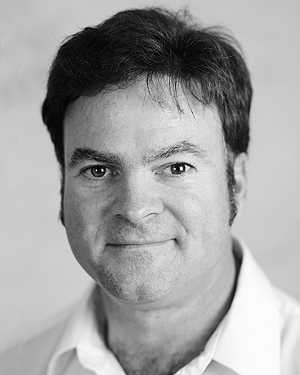
\includegraphics[width=1in,height=1.25in,clip,keepaspectratio]{a2.png}}]{Second B. Author} was born in Greenwich Village, New York, NY, USA in 
1977. He received the B.S. and M.S. degrees in aerospace engineering from 
the University of Virginia, Charlottesville, in 2001 and the Ph.D. degree in 
mechanical engineering from Drexel University, Philadelphia, PA, in 2008.

From 2001 to 2004, he was a Research Assistant with the Princeton Plasma 
Physics Laboratory. Since 2009, he has been an Assistant Professor with the 
Mechanical Engineering Department, Texas A{\&}M University, College Station. 
He is the author of three books, more than 150 articles, and more than 70 
inventions. His research interests include high-pressure and high-density 
nonthermal plasma discharge processes and applications, microscale plasma 
discharges, discharges in liquids, spectroscopic diagnostics, plasma 
propulsion, and innovation plasma applications. He is an Associate Editor of 
the journal \emph{Earth, Moon, Planets}, and holds two patents. 

Dr. Author was a recipient of the International Association of Geomagnetism 
and Aeronomy Young Scientist Award for Excellence in 2008, and the IEEE 
Electromagnetic Compatibility Society Best Symposium Paper Award in 2011. 
\end{IEEEbiography}

\begin{IEEEbiography}[{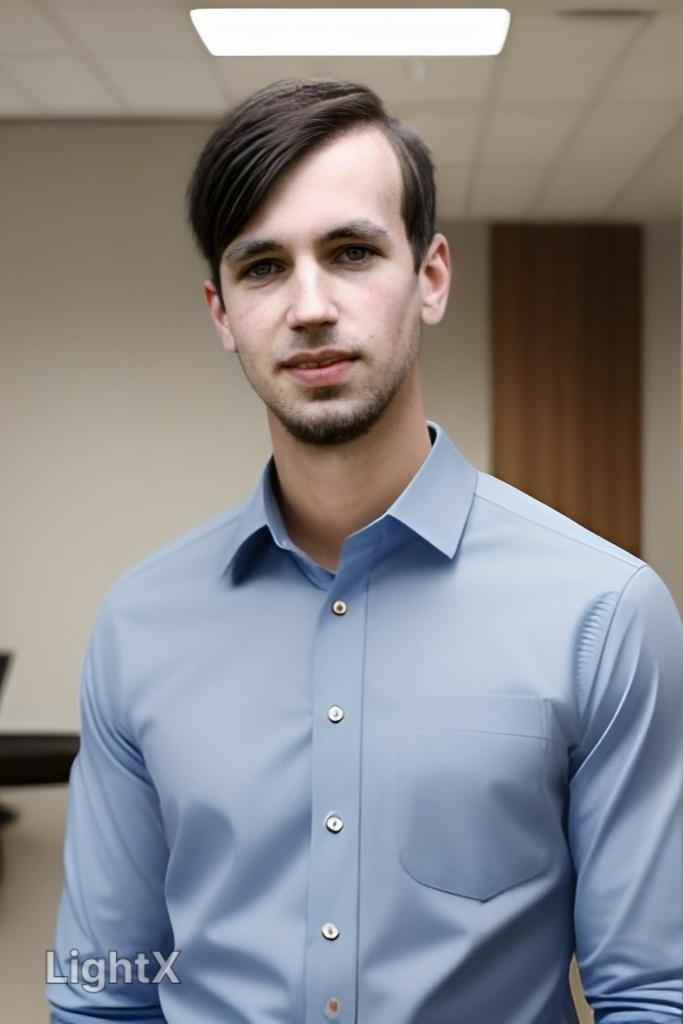
\includegraphics[width=1in,height=1.25in,clip,keepaspectratio]{a3.png}}]{Third C. Author, Jr.} (M'87) received the B.S. degree in mechanical 
engineering from National Chung Cheng University, Chiayi, Taiwan, in 2004 
and the M.S. degree in mechanical engineering from National Tsing Hua 
University, Hsinchu, Taiwan, in 2006. He is currently pursuing the Ph.D. 
degree in mechanical engineering at Texas A{\&}M University, College 
Station, TX, USA.

From 2008 to 2009, he was a Research Assistant with the Institute of 
Physics, Academia Sinica, Tapei, Taiwan. His research interest includes the 
development of surface processing and biological/medical treatment 
techniques using nonthermal atmospheric pressure plasmas, fundamental study 
of plasma sources, and fabrication of micro- or nanostructured surfaces. 

Mr. Author's awards and honors include the Frew Fellowship (Australian 
Academy of Science), the I. I. Rabi Prize (APS), the European Frequency and 
Time Forum Award, the Carl Zeiss Research Award, the William F. Meggers 
Award and the Adolph Lomb Medal (OSA).
\end{IEEEbiography}

\end{document}
